% ============================================================
%  第三卷 第十四章 角动量的相加（§106–§110 + §106 习题）
%  底本：高教社中文版第6版（严肃 译，喀兴林 校）；原书 pp.392–412
%  本章插图：图45（§108，四面体示意图，manifest p416）；表9、表10 为
%  公式表（非插图），按 tabular/数组重排。
%  正文圈码 20 处已全部转为 \footnote{}（脚注代理转录，见文件尾记录）。
%
%  已修正的 OCR / 原书错误（均对照 原书转换/pages/p-405…p-425.png 核实）：
%  1. (106.1) 按原书 p392 重建：指标组上的秩记号 2j₁、2j₂ 以 \overbrace 排出；
%  2. (106.2) OCR "{\bf\zeta}({\bf\zeta}-1)^{j-m}" → (-1)^{j-m}；
%  3. 直积分解式末项 OCR "D^{((j_1-j_2))}" → 按原书 D^{(|j_1-j_2|)}；
%  4. (106.4) 前不等式之后及 (106.5) 式尾的 OCR 乱码按原书均为“等等”；
%  5. (106.11) 逆变换系数 OCR 误作 ⟨j₁,m₁+m₂|m₁m₂⟩，按物理意义与 p395 排为
%     ⟨j, m₁+m₂|m₁m₂⟩（bra 的第一个记号为求和指标 j）；
%  6. (106.12)(106.13) OCR 中间步骤的 3j 符号完全乱版，按原书 p396 重建
%     （两式均无附加相因子；跨页断行已合并）；
%  7. (106.14) 按原书 p396 重建：求和相位 (-1)^{z+j₁-j₂-m₃}，分母六个阶乘；
%  8. (106.17) OCR 分子漏 (2j₂)!(j₁+j₂±m₁+m₂)! 等、分母末因子误作
%     (j₂-m₁-m₂)!，按原书 p397 为 (2j₂)!…(j₂-m₂)!，已补正；
%     其后未编号的 (j₁ j₂ j₃; j₁ −j₁−m₃ m₃) 公式按原书重建；
%  9. §106 习题解：3j 符号 (l ½ j; m−σ σ −m)，OCR 误作 (l 1 2)；
%     结果第二行 ψ_{l-1/2,m} 按原书；
% 10. 表9 整表（j₃=1/2,1,3/2,2 各块）OCR 为公式图片+乱码 HTML，按原书
%     p397–399 全部重建；表头对角线记号 m₃╲j₁ 以 \backslash 近似；
% 11. §107 (107.2) f₂₀ 的张量分量 OCR 误作 a_xx，按原书 p400 为 -√(3/2)a_zz；
%     f_{2,±1}、f_{2,±2} 的系数（无 √(3/2) 因子）按原书；
% 12. (107.3) 下标 OCR κϱ → KQ（希腊字母误读）；
% 13. §108 (108.2) 6j 定义式 OCR 误为 \int_{j_4}^{j_1}…，按原书 p403 重建
%     （≡ 号、求和下标“所有m”、相位 \sum_i(j_i-m_i)）；
% 14. (108.7) OCR 完全乱版，按原书 p405 重建：
%     Σ_j(2j+1)(2j″+1){j₁ j₂ j′;j₃ j₄ j}{j₃ j₂ j;j₁ j₄ j″}=δ_{jj″}；
% 15. (108.9) 三个 6j 符号连乘公式 OCR 乱版，按原书 p406 重建；
% 16. (108.10) 四个 Δ 因子按原书为 Δ(j₁j₂j₃)Δ(j₁j₅j₆)Δ(j₄j₂j₆)Δ(j₄j₅j₃)；
% 17. 表10 整表 OCR 完全乱码，按原书 p407 重建全部 7 个公式（含 s=a+b+c）；
% 18. (108.11) 求和下标 OCR 误作 Σ_{j₁₁}，按原书为对所有 m 求和；(108.12)
%     相位 (-1)^{2j} 及三个 6j 符号的排列按原书 p408；
% 19. §109 (109.2) 前的推导式按原书 p409 放大核实重建：求和记号 Σ_{m₁m₁′}，
%     相因子 (-1)^{j′₁-j₂+M′-M}（OCR 丢撇号）；两个 3j 符号中的 m₂ 均为
%     普通记号（草稿误加 Landau 求和点，原书无点，已改回）；
% 20. (109.5) 6j 符号 {J j₂′ j₁′;k j₁ j₂} 及两个约化矩阵元的撇号按原书 p410
%     （OCR 撇号丢失）；
% 21. §110 末段 (110.3) 特例积分：原书 p412 印作 sin α dα dβ /4π，按欧拉角
%     度规 dω=sinβ dα dβ dγ（(58.20)）及本页 α≡φ、β≡θ 的约定应为
%     sin β dα dβ，属原书排印错误，已改正；
% 22. §110 (110.6) 中的 ⟨μ′|f_{kq′}|μ⟩ OCR 误作 f_{kq}，按原书补撇号；
%     e^{im′γ} OCR 误作 e^{im′y}；
% 23. §110 (110.1) 第二个 D 函数下标 OCR/原书版面模糊作 m₂m₂，按 (106.11)
%     的转动关系应为 m′₂m₂，已排作 m′₂m₂；
% 24. 其它：\mathrm{d} 收紧、函数名 \sin\cos 正体、行内公式与中文粘连拆开、
%     半角标点按文体约定改全角（数学环境内保持 ASCII）。
%
%  遗留问题（OCR/原书存疑，已照原书排版）：
%  - (106.11) bra 首记号原书版面疑为 j₁（p395），因与求和指标矛盾按 j 排；
%  - (109.2) 前推导式的相因子 (-1)^{j′₁-j₂+M′-M} 照原书 p409 排（其相位
%    约定与 (106.10) 的定义有关，未改动）；
%  - (106.7)、(106.10)、(106.11)、(110.7) 式尾原书即无标点，照排；
%  - 表9/表10 的整表框线与对角线表头按原书近似重建（原书为正式排表格）。
%
%  脚注转录（脚注代理，对照 原书转换/pages300/p-405…p-424.png 页底脚注区）：
%  - 全章圈码 20 处全部转为 \footnote{}。脚注所在 PDF 物理页：p405(×2),408(×2),
%    409,410(×2),413(×2),414(×3),415,417(×3),419,420,421,424；
%  - 含公式的脚注：§106 脚注②（时间反演式 ψ_jm→(−1)^{j−m}ψ_{j,−m}）、§106
%    C-G 系记录号式（C^{jm}_{m₁m₂} 或 C^{jm}_{j₁m₁,j₂m₂}）、§108 W 符号与 6j
%    记号关系式；§106 脚注①含两段（\par 分段）；
%  - p414 脚注①末“(f₁g₁)₀₀=A·B 秩”之“秩”系原书排印疑误（语义应为“积”/
%    标积），照原书录作“秩”；p421 脚注俄文两书（Юцис 等、Варшалович 等）
%    书名、出版地照录，原书“——М. : Наука”冒号前空格收紧；p409 脚注 Edmonds
%    书名原书为斜体，本重排按章内无 textit 体例排正体.
%  - 包7复核：对照 pages300 p405–p425 各页页底逐条核实（p406/407/411/412/
%    416/418/422/423/425 无脚注区，p425 为空白章尾页），20 处转录逐字忠实、
%    无遗漏（脚注页码对照.txt 本章仅检出 14 个标记，系 OCR 形态漏检，以页面
%    实况为准）；smoke 编译（xelatex, jobname=smokefn_ch14）0 Error、无
%    overfull，smoke 文件用后已删.
% ============================================================
\chapter{角动量的相加}

\section{\texorpdfstring{$3j$}{3j} 符号}

§31中导出的角动量相加法则，给出了角动量为 $j_1$ 和 $j_2$ 的两个粒子（或两个更复杂的部分）所组成\footnote{严格讲来，我们总是考虑这样一个系统（以后不必每次声明），它的各部分之间相互作用很弱，以致每部分的角动量在一级近似下可以看作是守恒的.\par 下面所得的全部结果，当然不但能应用于两个粒子（或粒子系统）的总角动量的相加，而且也能应用于同一系统的轨道角动量和自旋的相加，假如自旋-轨道耦合是足够弱的话.}系统总角动量的各种可能值.这个法则实际上和波函数的空间旋转性质密切相关，并可根据旋量的性质立即得出.

角动量为 $j_1$ 和 $j_2$ 的粒子波函数分别是 $2j_1$ 秩和 $2j_2$ 秩的对称旋量，系统的波函数则等于它们的乘积：
\begin{equation}
  \psi^{(1)}\overbrace{\lambda\mu\cdots}^{2j_1}\ \
  \psi^{(2)}\overbrace{\rho\sigma\cdots}^{2j_2}.
\end{equation}
这个乘积对所有的指标对称化后，得到一个 $2(j_1+j_2)$ 秩的对称旋量，对应于总角动量为 $j_1+j_2$ 的态.如果我们把乘积(106.1)中的一对指标缩并掉，其中的一个指标取自 $\psi^{(1)}$ 另一个指标取自 $\psi^{(2)}$（否则缩并后等于零），由于 $\psi^{(1)}$ 和 $\psi^{(2)}$ 都是对称旋量，$\lambda,\mu,\cdots$ 和 $\rho,\sigma,\cdots$ 中不管取哪一对指标进行缩并都是一样的，经过对称化以后，得到一个 $2(j_1+j_2-1)$ 秩的旋量，对应于角动量为 $j_1+j_2-1$ 的态\footnote{为避免误解，作下列说明是有益的.双粒子系统的波函数永远是一个 $2(j_1+j_2)$ 秩的旋量，这个秩数一般地不等于 $2j$，$j$ 是该系统的总角动量.但是，这个旋量可以等价于一个低秩旋量.例如，角动量 $j_1=j_2=\frac{1}{2}$ 的双粒子系统波函数是一个 2 秩旋量.但如总角动量 $j=0$，这个旋量是反对称的，因而可化成一个标量.一般讲来，总角动量 $j$ 确定了该系统旋量波函数的对称性：它对 $2j$ 个指标是对称的并对其余指标反对称.}.继续这种手续，可得从 $j_1+j_2$ 直到 $|j_1-j_2|$ 的 $j$ 值各一次，和已知的角动量相加法则相一致.

从数学上讲来，这就是把旋转群两个不可约表示（$2j_1+1$ 维和 $2j_2+1$ 维）的直积 $D^{(j_1)}\times D^{(j_2)}$ 分解为不可约成分，于是角动量的相加法则可写成
\begin{equation*}
  D^{(j_1)}\times D^{(j_2)}
  =D^{(j_1+j_2)}+D^{(j_1+j_2-1)}+\cdots+D^{(|j_1-j_2|)}.
\end{equation*}
为了完全解决角动量相加问题，我们还须研究怎样由两个组成粒子的波函数构造具有给定总角动量值的系统波函数问题.

我们先从简单情形开始，亦即两个角动量相加后所得的总角动量等于零的情形.此时显然有 $j_1=j_2$ 以及角动量分量 $m_1=-m_2$.令 $\psi_{jm}$ 为一个粒子的归一化状态波函数（呈非旋量形式）；它具有角动量 $j$ 和分量 $m$.所求的系统波函数 $\psi_0$，等于 $m$ 值相反的两个粒子波函数的乘积之和：
\begin{equation}
  \psi_0=\frac{1}{\sqrt{2j+1}}\sum_{m=-j}^{j}(-1)^{j-m}
  \psi^{(1)}_{jm}\psi^{(2)}_{j,-m},
\end{equation}
$j$ 等于 $j_1$ 和 $j_2$ 的公共值.求和式前的因子来自归一化.求和式中的各个系数必须具有相同的绝对值，因为所有的角动量分量值 $m$ 应该是等概率的.(106.2)式中的符号序次很易用波函数的旋量形式求出.采用旋量记号，(106.2)中的求和式为下列标量（系统总角动量为零）
\begin{equation}
  \psi^{(1)\lambda\mu\cdots}\psi^{(2)}_{\lambda\mu\cdots},
\end{equation}
它是由两个 $2j$ 秩旋量所组成.根据上式，我们可从(57.3)式直接求出(106.2)式中各项的符号.

但应注意，一般讲来我们只能确定求和式(106.2)中各项的相对符号，至于整个求和式的符号则可能与角动量的“相加次序”有关.实际上，如果把 $\psi^{(1)}$ 中所有的旋量指标全部下降（有 $j+m$ 个指标为 1，$j-m$ 个指标为 2）并把 $\psi^{(2)}$ 中的指标全部上升，(106.3) 的标量就要乘以 $(-1)^{2j}$，当 $j$ 为半整数时就要变一符号.

其次，我们来考虑总角动量为零的一个系统，由角动量为 $j_1,j_2,j_3$ 分量为 $m_1,m_2,m_3$ 的三个粒子所组成.总角动量等于零的条件是 $m_1+m_2+m_3=0$，并且 $j_1,j_2,j_3$ 中任意一个的值可以从其它两个值的矢量相加法则中得到，也就是说，$\boldsymbol{j}_1,\boldsymbol{j}_2,\boldsymbol{j}_3$ 在几何上应该是一个封闭三角形的三条边.换句话说，每一个值介于其它两值的和与差之间：
\begin{equation*}
  |j_1-j_2|\leqslant j_3\leqslant j_1+j_2,\ \text{等等}
\end{equation*}
代数和 $j_1+j_2+j_3$ 显然是一个整数.

所考虑系统的波函数为下列求和式：
\begin{equation}
  \psi_0=\sum_{m_1,m_2,m_3}
  \left(\begin{array}{ccc}j_1&j_2&j_3\\m_1&m_2&m_3\end{array}\right)
  \psi^{(1)}_{j_1m_1}\psi^{(2)}_{j_2m_2}\psi^{(3)}_{j_3m_3},
\end{equation}
每个 $j_i$ 的取值是从 $-j_i$ 到 $j_i$.这个公式中的系数称为维格纳（Wigner）$3j$ 符号.按定义仅当 $m_1+m_2+m_3=0$ 时它们才不等于零.

置换下标 1,2,3 时，(106.4)式的波函数只能改变一个不重要的周相因子.实际上 $3j$ 符号可以全部定义成实量（见后面），$\psi_0$ 的不确定性就变成只是它的公共符号的不确定性（正如(106.2)式的函数那样）.这意味着 $3j$ 符号中列的对换使它或者不变或者变一符号.

确定求和式(106.4)中系数（3j 符号的常用定义）的一个最对称的方法是这样的.采用旋量记号，$\psi_0$ 是由三个旋量 $\psi^{(1)\lambda\mu\cdots},\psi^{(2)\lambda\mu\cdots},\psi^{(3)\lambda\mu\cdots}$ 的乘积经过全部指标的缩并后形成的一个标量，每一对缩并指标取自其中的两个不同旋量.对粒子 1 和 2 讲来，缩并时 $\psi^{(1)}$ 取上标 $\psi^{(2)}$ 取下标；对粒子 2 和 3，缩并时 $\psi^{(2)}$ 取上标 $\psi^{(3)}$ 取下标；对粒子 3 和 1，则 $\psi^{(3)}$ 取上标 $\psi^{(1)}$ 取下标.很易证明，这三类缩并指标分别有 $j_1+j_2-j_3$，$j_2+j_3-j_1$ 和 $j_1+j_3-j_2$ 对.这个缩并规则唯一地确定了 $\psi_0$ 的符号.

显然，采用了这个定义以后，指标 1,2,3 的循环置换使 $\psi_0$ 保持不变.这意味着 $3j$ 符号对列的循环置换保持不变.很易看出，1,2,3 中任意两个指标的对换，会使 $j_1+j_2+j_3$ 对旋量指标发生升降，这意味着 $\psi_0$ 要乘以 $(-1)^{j_1+j_2+j_3}$；换句话说，$3j$ 符号具有下列性质：
\begin{equation}
  \left(\begin{array}{ccc}j_2&j_1&j_3\\m_2&m_1&m_3\end{array}\right)
  =(-1)^{j_1+j_2+j_3}
  \left(\begin{array}{ccc}j_1&j_2&j_3\\m_1&m_2&m_3\end{array}\right)\ \text{等等，}
\end{equation}
即当 $j_1+j_2+j_3$ 为奇数时，任意两列的对调要变一符号.

最后，很易看出
\begin{equation}
  \left(\begin{array}{ccc}j_1&j_2&j_3\\-m_1&-m_2&-m_3\end{array}\right)
  =(-1)^{j_1+j_2+j_3}
  \left(\begin{array}{ccc}j_1&j_2&j_3\\m_1&m_2&m_3\end{array}\right),
\end{equation}
每个角动量 $z$ 分量的变号可看作绕 $y$ 轴转 $\pi$ 角的结果，这等价于把所有的旋量下标上升并同时把所有的上标下降（见(58.5)式）.

从(106.4)式出发，可以导出一个重要公式，这个公式能够给出具有给定 $j$ 和 $m$ 值的双粒子系统的 $\psi_{jm}$ 波函数，为此，我们把粒子 1 和 2 一起看作一个系统.由于这个系统的角动量 $\boldsymbol{j}$ 和粒子 3 的角动量 $\boldsymbol{j}_3$ 相加后所得的总角动量等于零，故一定有 $j=j_3$，$m=-m_3$.按(106.2)，我们可写成
\begin{equation}
  \psi_0=\frac{1}{\sqrt{2j+1}}\sum_m(-1)^{j-m}
  \psi_{jm}\psi^{(3)}_{j,-m}
\end{equation}
此式应该和(106.4)式比较（该式中的 $j_3$，$m_3$ 改成 $j$，$-m$）.在这里，我们首先要计及这样的事实，(106.7)中的求和是按(106.3)式的构造法则进行的，与(106.4)的求和式的构造法则并不一致；为了把(106.7)化成(106.4)的形式，不难看出，我们必须把粒子 1 和 3 的每对缩并指标上下对调一下，这就产生了一个附加因子 $(-1)^{j_1-j_2+j_3}$.比较的结果为\footnote{根据(60.2)式，时间反演下，波函数变成
\begin{equation*}
  \psi_{jm}\to(-1)^{j-m}\psi_{j,-m}
\end{equation*}
很易验证，(106.8)式的右边确实同其左边一样按上式变换的.}
\begin{equation}
  \psi_{jm}=(-1)^{j_1-j_2+m}\sqrt{2j+1}\sum_{m_1,m_2}
  \left(\begin{array}{ccc}j_1&j_2&j\\m_1&m_2&-m\end{array}\right)
  \psi^{(1)}_{j_1m_1}\psi^{(2)}_{j_2m_2},
\end{equation}
式中对 $m_1,m_2$ 的求和应满足 $m_1+m_2=m$ 的条件.

(106.8)式给出了我们所需要的表式，它把角动量为 $j_1$ 和 $j_2$ 的两个粒子波函数组合成为系统的波函数.该式可写成
\begin{equation}
  \psi_{jm}=\sum_{m_1,m_2}\langle m_1m_2|jm\rangle
  \psi^{(1)}_{j_1m_1}\psi^{(2)}_{j_2m_2}
  \quad(m_2=m-m_1),
\end{equation}
式中的系数
\begin{equation}
  \langle m_1m_2|jm\rangle=(-1)^{j_1-j_2+m}\sqrt{2j+1}
  \left(\begin{array}{ccc}j_1&j_2&j\\m_1&m_2&-m\end{array}\right)
\end{equation}
\emergencystretch=2em%
组成一个变换矩阵，它把 $(2j_1+1)(2j_2+1)$ 个正交归一化的完备波函数 $|m_1m_2\rangle$ 变换成为同样完备的 $|jm\rangle$ 波函数组（具有给定的 $j_1,j_2$ 值）.这种系数称为矢量耦合系数或克莱布什-高丹（Clebsch-Gordan）系数.记号 $\langle m_1m_2|jm\rangle$ 就是一组函数展为另一组函数时常用的(11.18)式中的展开系数的记号.为简洁计，我们已在记号中省略了两组函数共有的量子数 $j_1$ 和 $j_2$.必要时可恢复成 $\langle j_1m_1j_2m_2|j_1j_2jm\rangle$ \footnote{克莱布什-高丹系数（C-G 系数）在有的文献中记作
\begin{equation*}
  C_{m_1m_2}^{jm}\qquad\text{或}\qquad C_{j_1m_1,j_2m_2}^{jm}.
\end{equation*}}\par
\emergencystretch=0pt%

(106.9)的变换矩阵是幺正的（见§12）.因此逆变换系数
\begin{equation}
  \psi^{(1)}_{j_1m_1}\psi^{(2)}_{j_2m_2}
  =\sum_{j=|j_2-j_1|}^{j_1+j_2}\langle j,\,m_1+m_2|m_1m_2\rangle
  \psi_{j,m_1+m_2}
\end{equation}
等于(106.9)式中变换系数的复共轭.后面将指出，这些系数都是些实量，因此简单地有
\begin{equation*}
  \langle m_1m_2|jm\rangle=\langle jm|m_1m_2\rangle.
\end{equation*}
根据量子力学的一般规则，(106.11)中展开系数的平方给出了系统具有某个 $j$ 和 $m$ 值的概率（当 $j_1,m_1$ 和 $j_2,m_2$ 为给定时）.

变换(106.9)的幺正性意味着它的系数满足一定的正交条件.根据(12.5) 和(12.6)式有
\begin{equation}
\begin{aligned}
  \sum_{m_1,m_2}\langle m_1m_2|jm\rangle\langle m_1m_2|j'm'\rangle
  ={}&(2j+1)\sum_{m_1,m_2}
  \left(\begin{array}{ccc}j_1&j_2&j\\m_1&m_2&-m\end{array}\right)
  \left(\begin{array}{ccc}j_1&j_2&j'\\m_1&m_2&-m'\end{array}\right)=\\
  ={}&\delta_{jj'}\delta_{mm'},
\end{aligned}
\end{equation}
\begin{equation}
\begin{aligned}
  \sum_j\langle m_1m_2|jm\rangle\langle m_1'm_2'|jm\rangle
  ={}&\sum_j(2j+1)
  \left(\begin{array}{ccc}j_1&j_2&j\\m_1&m_2&-m\end{array}\right)
  \left(\begin{array}{ccc}j_1&j_2&j\\m_1'&m_2'&-m\end{array}\right)=\\
  ={}&\delta_{m_1m_1'}\delta_{m_2m_2'}.
\end{aligned}
\end{equation}

$3j$ 符号的一般显示表达式是相当冗长的.它可写成\footnote{(106.9)式中的系数由维格纳（E.~P.~Wigner, 1931）首先算出.它的对称性质及对称表式(106.14)由拉卡（G.~Racah, 1942）首先导出.最直接的导出方法也许是利用(57.6)式把 $\psi_0$ 的旋量表式（加以适当的归一化后）直接化成(106.4)的求和式.注意(57.6)中的系数是实的，因此 $3j$ 符号也一定是实数.另一种推导见 A.~R.~Edmonds, Angular Momentum in Quantum Mechanics, Princeton, 1957. 后面的 $3j$ 符号表引自此书.}
\begin{equation}
\begin{aligned}
  \left(\begin{array}{ccc}j_1&j_2&j_3\\m_1&m_2&m_3\end{array}\right)
  ={}&\left[\frac{(j_1+j_2-j_3)!\ (j_1-j_2+j_3)!\ (-j_1+j_2+j_3)!}{(j_1+j_2+j_3+1)!}\right]^{1/2}\times\\
  &\times\left[(j_1+m_1)!\ (j_1-m_1)!\ (j_2+m_2)!\ (j_2-m_2)!\ (j_3+m_3)!\ (j_3-m_3)!\right]^{1/2}\times\\
  &\times\sum_z\tfrac{(-1)^{z+j_1-j_2-m_3}}{z!\ (j_1+j_2-j_3-z)!\ (j_1-m_1-z)!\ (j_2+m_2-z)!\ (j_3-j_2+m_1+z)!\ (j_3-j_1-m_2+z)!}
\end{aligned}
\end{equation}
式中对所有的整数 $z$ 值求和，但由于负整数的阶乘为无穷大，这个求和式中只有为数有限的项.求和式前的系数明显对称于下标 1,2,3；把求和变量 $z$ 的值变换一下即可看出求和式本身也具有这种对称性.

除了根据 $3j$ 符号的定义直接导出的对称性质(106.5)和(106.6)式以外，$3j$ 符号还存在着其它一些对称性质，但它们的推导较为复杂，我们不在这里给出.所讲的这些对称性可用 $3j$ 符号的参量所组成的下列 $3\times3$ 数值表很好地表达出来：
\begin{equation}
  \left(\begin{array}{ccc}j_1&j_2&j_3\\m_1&m_2&m_3\end{array}\right)
  =\left[\begin{array}{ccc}
  j_2+j_3-j_1 & j_3+j_1-j_2 & j_1+j_2-j_3\\
  j_1-m_1 & j_2-m_2 & j_3-m_3\\
  j_1+m_1 & j_2+m_2 & j_3+m_3
  \end{array}\right],
\end{equation}
此表中每行或每列之和都等于 $j_1+j_2+j_3$.然后有：（1）表中任意两列对调后，$3j$ 符号要乘以 $(-1)^{j_1+j_2+j_3}$（与(106.5)所给的性质相同）；（2）任意两行对调后同样要乘以 $(-1)^{j_1+j_2+j_3}$（对下面两行讲来，与(106.6)所给的性质相同）；（3）表中的行和列对调后 $3j$ 符号保持不变\footnote{见 T.~Regge, Il nuovo cimento 10, 544, 1958; 11, 116, 1959. (106.15)对称性（以及 $6j$ 符号(108.3)式的性质）的更深入的数学特征的讨论见评述性文章 Я.~А.~Смородинский и Л.~А.~Шелепин, УФН, 106, 3 (1972).}.

下面给出特殊情形下的某些简单公式.按(106.2)有下列数值：
\begin{equation}
  \left(\begin{array}{ccc}j&j&0\\m&-m&0\end{array}\right)
  =(-1)^{j-m}\frac{1}{\sqrt{2j+1}}.
\end{equation}
由(106.14)式直接可得：
\begin{equation}
\begin{aligned}
  \left(\begin{array}{ccc}j_1&j_2&j_1+j_2\\m_1&m_2&-m_1-m_2\end{array}\right)
  ={}&(-1)^{j_1-j_2+m_1+m_2}\times\\
  &\times\left[\tfrac{(2j_1)!\ (2j_2)!\ (j_1+j_2+m_1+m_2)!\ (j_1+j_2-m_1-m_2)!}
  {(2j_1+2j_2+1)!\ (j_1+m_1)!\ (j_1-m_1)!\ (j_2+m_2)!\ (j_2-m_2)!}\right]^{1/2}
\end{aligned}
\end{equation}
\begin{equation*}
\begin{aligned}
  \left(\begin{array}{ccc}j_1&j_2&j_3\\j_1&-j_1-m_3&m_3\end{array}\right)
  ={}&(-1)^{-j_1+j_2+m_3}\times\\
  &\times\left[\tfrac{(2j_1)!\ (-j_1+j_2+j_3)!\ (j_1+j_2+m_3)!\ (j_3-m_3)!}
  {(j_1+j_2+j_3+1)!\ (j_1-j_2+j_3)!\ (j_1+j_2-j_3)!\ (-j_1+j_2-m_3)!\ (j_3+m_3)!}\right]^{1/2}
\end{aligned}
\end{equation*}
下列公式
\begin{equation}
\begin{aligned}
  \left(\begin{array}{ccc}j_1&j_2&j_3\\0&0&0\end{array}\right)
  ={}&(-1)^p\left[\frac{(j_1+j_2-j_3)!\ (j_1-j_2+j_3)!\ (-j_1+j_2+j_3)!}{(2p+1)!}\right]^{1/2}\times\\
  &\times\frac{p!}{(p-j_1)!\ (p-j_2)!\ (p-j_3)!}
\end{aligned}
\end{equation}
当 $2p=j_1+j_2+j_3$ 为偶数时，上式的推导需要许多附加计算\footnote{见前引 Edmonds 的书.}，当 $2p$ 为奇数时，这个 $3j$ 符号由于对称性(106.6)而等于零.

表 9 中列入了 $j_3=1/2,1,3/2,2$ 的各种 $3j$ 符号值，以供参考.对于每一个 $j_3$ 值，表中只给出了少数几个 $3j$ 符号，其余的 $3j$ 符号可以根据(106.5)，(106.6)式以及这个表推出.

\begin{center}
{\heiti 表 9}\quad $3j$ 符号表
\end{center}

\begin{equation*}
  \left(\begin{array}{ccc}j+\tfrac12&j&\tfrac12\\[2pt]m&-m-\tfrac12&\tfrac12\end{array}\right)
  =(-1)^{j-m-\frac12}\left[\frac{j-m-\tfrac12}{(2j+1)(2j+2)}\right]^{1/2}
\end{equation*}

\medskip\noindent\rule{\linewidth}{0.5pt}\medskip

\begin{equation*}
  (-1)^{j-m}\left(\begin{array}{ccc}j_1&j&1\\m&-m-m_3&m_3\end{array}\right)
\end{equation*}
\begin{center}
\renewcommand{\arraystretch}{1.7}%
\begin{tabular}{c|c}
  $m_3\ \backslash\ j_1$ & $0$\\ \hline
  $j$ & $\dfrac{2m}{\left[2j(2j+1)(2j+2)\right]^{1/2}}$\\[10pt]
  $j+1$ & $-\left[\dfrac{2(j+m+1)(j-m+1)}{(2j+1)(2j+2)(2j+3)}\right]^{1/2}$\\[10pt]
\end{tabular}

\medskip

\begin{tabular}{c|c}
  $m_3\ \backslash\ j_1$ & $1$\\ \hline
  $j$ & $\left[\dfrac{2(j-m)(j+m+1)}{2j(2j+1)(2j+2)}\right]^{1/2}$\\[10pt]
  $j+1$ & $-\left[\dfrac{(j-m)(j-m+1)}{(2j+1)(2j+2)(2j+3)}\right]^{1/2}$\\[10pt]
\end{tabular}
\end{center}

\medskip\noindent\rule{\linewidth}{0.5pt}\medskip

\begin{equation*}
  (-1)^{j-m+\frac12}\left(\begin{array}{ccc}j_1&j&\tfrac32\\m&-m-m_3&m_3\end{array}\right)
\end{equation*}
\begin{center}
\renewcommand{\arraystretch}{1.7}%
\begin{tabular}{c|c}
  $m_3\ \backslash\ j_1$ & $\tfrac12$\\ \hline
  $j+\tfrac12$ & $-\left(j+3m+\tfrac32\right)
  \left[\dfrac{j-m+\tfrac12}{2j(2j+1)(2j+2)(2j+3)}\right]^{1/2}$\\[10pt]
  $j+\tfrac32$ & $\left[\dfrac{3\left(j-m+\tfrac12\right)\left(j-m+\tfrac32\right)\left(j+m+\tfrac32\right)}
  {(2j+1)(2j+2)(2j+3)(2j+4)}\right]^{1/2}$\\[10pt]
\end{tabular}

\medskip

\begin{tabular}{c|c}
  $m_3\ \backslash\ j_1$ & $\tfrac32$\\ \hline
  $j+\tfrac12$ & $-\left[\dfrac{3\left(j-m-\tfrac12\right)\left(j-m+\tfrac12\right)\left(j-m+\tfrac32\right)}
  {2j(2j+1)(2j+2)(2j+3)}\right]^{1/2}$\\[10pt]
  $j+\tfrac32$ & $\left[\dfrac{\left(j-m-\tfrac12\right)\left(j-m+\tfrac12\right)\left(j-m+\tfrac32\right)}
  {(2j+1)(2j+2)(2j+3)(2j+4)}\right]^{1/2}$\\[10pt]
\end{tabular}
\end{center}

\medskip\noindent\rule{\linewidth}{0.5pt}\medskip

\begin{equation*}
  (-1)^{j-m}\left(\begin{array}{ccc}j_1&j&2\\m&-m-m_3&m_3\end{array}\right)
\end{equation*}
\begin{center}
\renewcommand{\arraystretch}{1.7}%
\begin{tabular}{c|c}
  $m_3\ \backslash\ j_1$ & $0$\\ \hline
  $j$ & $\dfrac{2\left[3m^2-j(j+1)\right]}{\left[(2j-1)2j(2j+1)(2j+2)(2j+3)\right]^{1/2}}$\\[10pt]
  $j+1$ & $-2m\left[\dfrac{6(j+m+1)(j-m+1)}{2j(2j+1)(2j+2)(2j+3)(2j+4)}\right]^{1/2}$\\[10pt]
  $j+2$ & $\left[\dfrac{6(j+m+2)(j+m+1)(j-m+2)(j-m+1)}
  {(2j+1)(2j+2)(2j+3)(2j+4)(2j+5)}\right]^{1/2}$\\[10pt]
\end{tabular}

\medskip

\begin{tabular}{c|c}
  $m_3\ \backslash\ j_1$ & $1$\\ \hline
  $j$ & $(1+2m)\left[\dfrac{6(j+m+1)(j-m)}
  {(2j-1)2j(2j+1)(2j+2)(2j+3)}\right]^{1/2}$\\[10pt]
  $j+1$ & $-2(j+2m+2)\left[\dfrac{(j-m+1)(j-m)}
  {2j(2j+1)(2j+2)(2j+3)(2j+4)}\right]^{1/2}$\\[10pt]
  $j+2$ & $2\left[\dfrac{(j+m+2)(j-m+2)(j-m+1)(j-m)}
  {(2j+1)(2j+2)(2j+3)(2j+4)(2j+5)}\right]^{1/2}$\\[10pt]
\end{tabular}

\medskip

\begin{tabular}{c|c}
  $m_3\ \backslash\ j_1$ & $2$\\ \hline
  $j$ & $\left[\dfrac{6(j-m-1)(j-m)(j+m+1)(j+m+2)}
  {(2j-1)2j(2j+1)(2j+2)(2j+3)}\right]^{1/2}$\\[10pt]
  $j+1$ & $-2\left[\dfrac{(j-m-1)(j-m)(j-m+1)(j+m+2)}
  {2j(2j+1)(2j+2)(2j+3)(2j+4)}\right]^{1/2}$\\[10pt]
  $j+2$ & $\left[\dfrac{(j-m-1)(j-m)(j-m+1)(j-m+2)}
  {(2j+1)(2j+2)(2j+3)(2j+4)(2j+5)}\right]^{1/2}$\\[10pt]
\end{tabular}
\end{center}

\begin{xiti}

\noindent{\heiti 习题}\quad 试求自旋为 $1/2$ 轨道角动量给定为 $l$ 的粒子态的角部波函数与总角动量为 $j$ 投影值为 $m$ 的状态波函数之间的关系.

解：这个问题可以用一般公式(106.8)解决，把该式中的 $\psi^{(1)}$ 理解为轨道角动量本征函数（即球谐函数 $\mathrm{Y}_{lm}$），把 $\psi^{(2)}$ 理解为自旋波函数 $\chi(\sigma)$［其中的 $\sigma=\pm\frac12$］：
\begin{equation*}
  \psi_{jm}=(-1)^{l+m-\frac12}\sqrt{2j+1}\sum_\sigma
  \left(\begin{array}{ccc}l&\tfrac12&j\\m-\sigma&\sigma&-m\end{array}\right)
  \mathrm{Y}_{l,m-\sigma}\chi(\sigma)
\end{equation*}
把 $3j$ 符号值代入后，即得：
\begin{equation*}
\begin{aligned}
  \psi_{l+\frac12,m}&=\sqrt{\frac{j+m}{2j}}\,
  \chi\left(\tfrac12\right)\mathrm{Y}_{l,m-\frac12}
  +\sqrt{\frac{j-m}{2j}}\,
  \chi\left(-\tfrac12\right)\mathrm{Y}_{l,m+\frac12}\\
  \psi_{l-\frac12,m}&=-\sqrt{\frac{j-m+1}{2j+2}}\,
  \chi\left(\tfrac12\right)\mathrm{Y}_{l,m-\frac12}
  +\sqrt{\frac{j+m+1}{2j+2}}\,
  \chi\left(-\tfrac12\right)\mathrm{Y}_{l,m+\frac12}
\end{aligned}
\end{equation*}

\end{xiti}

\section{张量的矩阵元}

§29中曾经得到过物理矢量的矩阵元与角动量分量值间的一些关系式.这些式子实际上不过是任意秩不可约张量（见§57）的某些相应的一般公式的一个特例\footnote{§107—§109中所分析的问题，大部分结果是由拉卡（G.~Racah, 1942—1943）给出的.}.

一个 $k$（整数）秩不可约张量的 $2k+1$ 个分量按其变换性质来说等价于 $2k+1$ 个球谐函数 $\mathrm{Y}_{kq}$，$q=-k,\cdots,k$（见§57最后一个附注），这就是说，把一个张量的分量适当地线性组合以后，我们可以得到一组量，这组量在转动下按函数组 $\mathrm{Y}_{kq}$ 的规律变换.我们用 $f_{kq}$ 代表这组量，称为 $k$ 秩球张量.

以 $k=1$ 的矢量为例，$f_{1q}$ 和矢量诸分量的关系式为
\begin{equation}
  f_{10}=\mathrm{i}a_z,\qquad
  f_{1,\pm1}=\mp\frac{\mathrm{i}}{\sqrt{2}}\,(a_x\pm\mathrm{i}a_y).
\end{equation}
参考(57.7).二秩张量的相应公式为
\begin{equation}
\left.\begin{aligned}
  f_{20}&=-\sqrt{\tfrac32}\,a_{zz},\qquad
  f_{2,\pm1}=\pm(a_{xz}\pm\mathrm{i}a_{yz}),\\
  f_{2,\pm2}&=-\tfrac12(a_{xx}-a_{yy}\pm2\mathrm{i}a_{xy}).
\end{aligned}\right\}
\end{equation}
且有 $a_{xx}+a_{yy}+a_{zz}=0$\footnote{之所以要取 $f_{kq}$ 为复量仅仅是因为我们采用的是球分量，而该张量原来的笛卡儿分量都是些实量.}.

两个（或更多个）球张量 $f_{k_1q_1},f_{k_2q_2}$ 可按角动量相加法则构造出张量乘积，$k_1$，$k_2$ 形式上代表着对应于这两个张量的“角动量”.因此可以按下式从 $k_1$ 和 $k_2$ 秩的两个球张量构造出 $K=k_1+k_2,\cdots,|k_1-k_2|$ 秩的球张量：
\begin{equation}
\begin{aligned}
  (f_{k_1}g_{k_2})_{KQ}=\sum_{q_1,q_2}\langle q_1q_2|KQ\rangle
  f_{k_1q_1}g_{k_2q_2}={}\\
  {}=(-1)^{k_1-k_2+Q}\sqrt{2K+1}\sum_{q_1,q_2}
  \left(\begin{array}{ccc}k_1&k_2&K\\q_1&q_2&-Q\end{array}\right)
  f_{k_1q_1}g_{k_2q_2}
\end{aligned}
\end{equation}
（参考(106.9)式）.但是，两个同为 $k$ 秩的张量的标积通常定义成为
\begin{equation}
  (f_kg_k)_{00}=\sum_q(-1)^{k-q}f_{kq}g_{k,-q},
\end{equation}
这个式子和 $K=Q=0$ 的(107.3)式相差一个因子 $\sqrt{2k+1}$，可参考(106.2)式\footnote{如果矢量 $\boldsymbol{A}$ 和 $\boldsymbol{B}$ 对应于(107.1)式的球张量 $f_{1q}$ 和 $g_{1q}$ 则有 $(f_1g_1)_{00}=\boldsymbol{A}\cdot\boldsymbol{B}$ 秩.}.这个定义也可改写成
\begin{equation*}
  (f_kg_k)_{00}=\sum_q f_{kq}g_{kq}^{*}.
\end{equation*}
如果我们注意到球张量的复共轭为\footnote{我们重复一下关于(106.8)式的说明：按此规则，对(107.3)式右边的两个 $k_1$ 和 $k_2$ 秩张量取复共轭，则使式左的 $K$ 秩张量也成为其复共轭.}（参考(28.9)）
\begin{equation*}
  f_{kq}^{*}=(-1)^{k-q}f_{k,-q}.
\end{equation*}
把物理量表成球张量的形式对其矩阵元的计算特别方便，这样一来就能直接应用角动量相加理论中的各种结果.

按矩阵元的定义，我们有
\begin{equation}
  \hat{f}_{kq}\psi_{njm}=\sum_{n'j'm'}
  \langle n'j'm'|f_{kq}|njm\rangle\psi_{n'j'm'},
\end{equation}
其中 $\psi_{njm}$ 为系统的定态波函数，该态由它的角动量 $j$，分量 $m$ 和其余量子数的集合 $n$ 所描写.(107.5)式左右两边的函数按其变换性质来说，分别对应于(106.11)式的两边，因此可以立刻得到以下一些选择定则：$k$ 秩不可约张量的 $f_{kq}$ 分量的矩阵元，除了满足“角动量相加法则”$j'=j+k$ 的 $jm\to j'm'$ 跃迁矩阵元外，其余都等于零，亦即量子数 $j',j,k$ 必须满足“三角形法则”（构成一个封闭三角形的三条边），并且有 $m'=m+q$.特别是，仅当 $2j\geqslant k$ 时，对角元才能不等于零.

其次，根据同样的变换对应，求和式(107.5)中的系数应该和(106.11)式中的系数成正比（维格纳-埃克特定理 Wigner-Eckart）.这一点确定了这些系数和 $m,m'$ 的关系，因此矩阵元可写成下列形式：
\begin{equation}
\begin{aligned}
  &\langle n'j'm'|f_{kq}|njm\rangle=\\
  &\quad=\mathrm{i}^k(-1)^{j_{\max}-m'}
  \left(\begin{array}{ccc}j'&k&j\\-m'&q&m\end{array}\right)
  \langle n'j'\Vert f_k\Vert nj\rangle,
\end{aligned}
\end{equation}
其中 $j_{\max}$ 代表 $j$ 和 $j'$ 二者中较大的那一个，$\langle n'j'\Vert f_k\Vert nj\rangle$ 是一些和 $m,m',q$ 无关的量，称为约化矩阵元.这个公式解决了矩阵元和角动量分量的依赖关系问题.这个关系完全是由对旋转群而言的对称性质所支配的，至于和其它量子数的关系则由 $f_{kq}$ 本身的物理特性所确定\footnote{根据这些结果，立刻可得 §29 中给出的矢量矩阵元的选择定则及其公式(29.7),(29.9).}.

算符组 $\hat{f}_{kq}$ 之间存在着下列关系:
\begin{equation}
  \hat{f}_{kq}^{+}=(-1)^{k-q}\hat{f}_{k,-q},
\end{equation}
因此对其矩阵元讲来，下式成立：
\begin{equation}
  \langle n'j'm'|f_{kq}|njm\rangle^{*}
  =(-1)^{k-q}\langle njm|f_{k,-q}|n'j'm'\rangle.
\end{equation}
把(107.6)代入上式并利用 $3j$ 符号的性质(106.5)和(106.6)，可得约化矩阵元的“厄米”关系\footnote{定义式(107.6)中的相因子实际上是这样选定的，使得(107.9)式成立.}：
\begin{equation}
  \langle n'j'\Vert f_k\Vert nj\rangle
  =\langle nj\Vert f_k\Vert n'j'\rangle^{*}.
\end{equation}
标量(107.4)的矩阵元对 $j$ 和 $m$ 是对角的.按矩阵乘法规则有
\begin{equation*}
\begin{aligned}
  &\langle n'jm|(f_kg_k)_{00}|njm\rangle=\\
  &\quad=\sum_q(-1)^{k-q}\sum_{n''j''m''}
  \langle n'jm|f_{kq}|n''j''m''\rangle
  \langle n''j''m''|g_{k,-q}|njm\rangle,
\end{aligned}
\end{equation*}
把(107.6)代入上式，利用 $3j$ 符号的正交关系对 $q$ 和 $m''$ 求和后，得到
\begin{equation}
  \langle n'jm|(f_kg_k)_{00}|njm\rangle
  =\frac{1}{2j+1}\sum_{n''j''}
  \langle n'j\Vert f_k\Vert n''j''\rangle
  \langle n''j''\Vert g_k\Vert nj\rangle.
\end{equation}
同理易得矩阵元平方和的下列公式
\begin{equation}
  \sum_{q,m'}|\langle n'j'm'|f_{kq}|njm\rangle|^2
  =\frac{1}{2j+1}\,|\langle n'j'\Vert f_k\Vert nj\rangle|^2,
\end{equation}
\begin{equation}
  \sum_{m,m'}|\langle n'j'm'|f_{kq}|njm\rangle|^2
  =\frac{1}{2k+1}\,|\langle n'j'\Vert f_k\Vert nj\rangle|^2.
\end{equation}
第一式是在给定 $m$ 值下对 $q$ 和 $m'$ 求和，第二式是在给定 $q$ 值下对 $m$ 和 $m'$ 求和（两式均有 $m'=m+q$）.

为参考计，我们来考察 $f_{kq}$ 就是球谐函数 $\mathrm{Y}_{kq}$ 本身时的情形，给出它对一个粒子的两个整数轨道角动量态 $l_1$ 和 $l_2$ 之间的跃迁矩阵元，即下列积分：
\begin{equation}
  \langle l_1m_1|\mathrm{Y}_{lm}|l_2m_2\rangle
  =\int \mathrm{Y}^{*}_{l_1m_1}\mathrm{Y}_{lm}\mathrm{Y}_{l_2m_2}\,\mathrm{d}o.
\end{equation}
除了角动量相加法则 $(l+l_2=l_1)$ 所赋予的选择定则以外，这个矩阵元还有一个 $l+l_1+l_2$ 必须为偶数的规则.这是来自宇称守恒，它要求两个粒子态的宇称乘积 $(-1)^{l_1+l_2}$ 必须等于所考虑物理量的宇称 $(-1)^l$（见§30）.

(107.13)式的那些矩阵元是§110 中所算的一个更普遍的积分的一个特例（是该节附注），它们由下式给出：
\begin{equation}
\begin{aligned}
  \langle l_1m_1|\mathrm{Y}_{lm}|l_2m_2\rangle
  ={}&(-1)^{m_1}\mathrm{i}^{-l_1+l_2+l}
  \left(\begin{array}{ccc}l_1&l&l_2\\-m_1&m&m_2\end{array}\right)\times\\
  &\times\left(\begin{array}{ccc}l_1&l&l_2\\0&0&0\end{array}\right)
  \left[\frac{(2l+1)(2l_1+1)(2l_2+1)}{4\pi}\right]^{1/2},
\end{aligned}
\end{equation}
特别是 $m_1=m_2=m=0$ 时，得三个勒让德函数的乘积积分式：
\begin{equation}
  \int_{-1}^{1}\mathrm{P}_l(\mu)\mathrm{P}_{l_1}(\mu)\mathrm{P}_{l_2}(\mu)\,\mathrm{d}\mu
  =2\left(\begin{array}{ccc}l_1&l&l_2\\0&0&0\end{array}\right)^{\!2}.
\end{equation}

\section{\texorpdfstring{$6j$}{6j} 符号}

§106中我们定义 $3j$ 符号为(106.4)式中对总角动量为零的三个粒子波函数求和时的系数.从旋转变换的性质讲来，这个和是一个标量，由于这一点，具有给定 $j_1,j_2,j_3$ 值（以及所有可能的 $m_1,m_2,m_3$ 值）的一组 $3j$ 符号可以看作这样一组量，它们在旋转下是按乘积 $\psi_{j_1m_1}\psi_{j_2m_2}\psi_{j_3m_3}$ 的逆步规律变换的，使得整个和是一个标量.

根据这个观点我们可以提出只用 $3j$ 符号构造标量的问题.这个标量必须只依赖于 $j$，不依赖于随转动变化的 $m$.换句话说，它必能表成对所有的 $m$ 求和的形式，这样的求和式就是两个 $3j$ 符号乘积的下列“缩并”式：
\begin{equation}
  \sum_m(-1)^{j-m}
  \left(\begin{array}{cc}j&\cdots\\m&\cdots\end{array}\right)
  \left(\begin{array}{cc}j&\cdots\\-m&\cdots\end{array}\right)
\end{equation}
［参考标量(106.2)的构造方法］.

由于每个“缩并”针对着一对 $m$，构造一个完整的标量时我们必须考虑偶数个 $3j$ 符号的乘积.两个 $3j$ 符号的乘积缩并时，由于其正交性，显然有
\begin{equation*}
\begin{aligned}
  \sum_{m_1,m_2,m_3}
  &\left(\begin{array}{ccc}j_1&j_2&j_3\\m_1&m_2&m_3\end{array}\right)
  \left(\begin{array}{ccc}j_1&j_2&j_3\\-m_1&-m_2&-m_3\end{array}\right)
  (-1)^{j_1+j_2+j_3-m_1-m_2-m_3}=\\
  &=\sum_{m_1,m_2,m_3}
  \left(\begin{array}{ccc}j_1&j_2&j_3\\m_1&m_2&m_3\end{array}\right)^{\!2}=1,
\end{aligned}
\end{equation*}
其中应用了等式 $m_1+m_2+m_3=0$ 及(106.6)，(106.12)式.因此构造一个非平凡标量所需的最少因子数等于 4.

每个 $3j$ 符号中，三个 $j$ 值组成一个封闭三角形.由于每个 $j$ 值必须出现在两个 $3j$ 符号的“缩并”中，显然，在用 4 个 $3j$ 符号的乘积构造一个标量时，一定会有 6 个 $j$ 值组成一个不规则四面体的 6 条棱（图45），每一个 $3j$ 符号对应于它的一个面.我们在定义所需的标量时，对其缩并过程照例要用一定的条件，它由下式给出：
\begin{equation}
\setlength{\arraycolsep}{3pt}%
\begin{aligned}
  \left\{\begin{array}{ccc}j_1&j_2&j_3\\j_4&j_5&j_6\end{array}\right\}
  \equiv\sum_{\text{所有}\,m}(-1)^{\sum_i(j_i-m_i)}
  &\left(\begin{array}{ccc}j_1&j_2&j_3\\-m_1&-m_2&-m_3\end{array}\right)\times\\
  \times&\left(\begin{array}{ccc}j_1&j_5&j_6\\m_1&-m_5&m_6\end{array}\right)
  \left(\begin{array}{ccc}j_4&j_2&j_6\\m_4&m_2&-m_6\end{array}\right)
  \left(\begin{array}{ccc}j_4&j_5&j_3\\-m_4&m_5&m_3\end{array}\right),
\end{aligned}
\end{equation}
\par\nopagebreak\noindent\begin{minipage}{\linewidth}\centering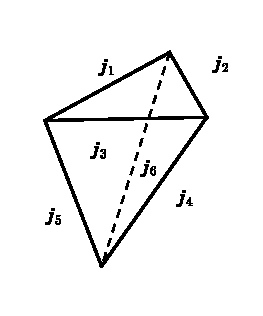
\includegraphics[width=4cm]{fig45.pdf}\\[0.3em]{\small 图 45}\end{minipage}\par\nopagebreak
式中对所有 $m$ 的所有可能值求和，但由于每个 $3j$ 符号中的三个 $m$ 值之和必须为零，6 个 $m$ 中实际上只有 3 个 $m$ 是独立的，(108.2)式所定义的量称为 $6j$ 符号或拉卡系数\footnote{文献中也有的用下列记号
\begin{equation*}
  W(j_1j_2j_4j_5;j_3j_6)=(-1)^{j_1+j_2+j_4+j_5}
  \left\{\begin{array}{ccc}
    j_1 & j_2 & j_3 \\
    j_4 & j_5 & j_6
  \end{array}\right\}.
\end{equation*}}.

根据定义(108.2)，应用 $3j$ 符号的对称性质，不难验证 $6j$ 符号中的三列进行任意置换时，或者任意两列的上下指标同时对调时，$6j$ 符号保持不变.由于这些对称性质，$6j$ 符号中的 $j_1,\cdots,j_6$ 可以排列成 24 种等价的形式\footnote{如果把图45看作一个正四面体，那么 $j$ 的 24 种等价置换可以从该四面体的 24 种对称变换（旋转和反射）获得.}.此外，$6j$ 符号还有一个不太明显的对称性质，这是两组不同 $j$ 值的符号间的一个等式\footnote{见 T.~Regge, Il nuovo cimento [10] 10, 544, 1958; 11, 116, 1959.}：
\begin{equation}
\begin{aligned}
  &\left\{\begin{array}{ccc}j_1&j_2&j_3\\j_4&j_5&j_6\end{array}\right\}=\\
  &\quad=\left\{\begin{array}{ccc}
  j_1 & \tfrac12(j_2+j_5+j_3-j_6) & \tfrac12(j_3+j_6+j_2-j_5)\\
  j_4 & \tfrac12(j_2+j_5+j_6-j_3) & \tfrac12(j_3+j_6+j_5-j_2)
  \end{array}\right\}.
\end{aligned}
\end{equation}
下面给出 $6j$ 符号与 $3j$ 符号间一个有用的关系式，它可从定义(108.2)导出：
\begin{equation}
\begin{aligned}
  \sum_{m_4m_5m_6}&(-1)^{j_4+j_5+j_6-m_4-m_5-m_6}
  \left(\begin{array}{ccc}j_1&j_5&j_6\\m_1&-m_5&m_6\end{array}\right)\times\\
  &\times\left(\begin{array}{ccc}j_4&j_2&j_6\\m_4&m_2&-m_6\end{array}\right)
  \left(\begin{array}{ccc}j_4&j_5&j_3\\-m_4&m_5&m_3\end{array}\right)
  =\left(\begin{array}{ccc}j_1&j_2&j_3\\m_1&m_2&m_3\end{array}\right)
  \left\{\begin{array}{ccc}j_1&j_2&j_3\\j_4&j_5&j_6\end{array}\right\},
\end{aligned}
\end{equation}
式左的求和项与(108.2)中的相比少了一个 $3j$ 符号.因此我们可以说，(108.4)中的和可用缺掉一个面的四面体（图45）代表.这一点确定了它与标量求和式的差别.换句话说，就其变换性质而言，它相当于一个 $3j$ 符号，这个符号一定和(108.4)式右边的那个 $3j$ 符号成正比.该式两边乘以
\begin{equation*}
  \left(\begin{array}{ccc}j_1&j_2&j_3\\m_1&m_2&m_3\end{array}\right)
\end{equation*}
并对 $m_1,m_2,m_3$ 求和后，很易求出其比例系数（即该式右边的 $6j$ 符号）.

$6j$ 符号在下述三个角动量的相加问题中自然地产生.

设 $j_1,j_2,j_3$ 三个角动量相加后给出的总角动量为 $J$.当 $J$ 值（及其分量值 $M$）给定后，该系统的态还没有唯一地确定，它还依赖于这些角动量相加的方式（或称耦合方案）.

例如，我们来考虑这样两个耦合方案：（1）先把角动量 $j_1$ 和 $j_2$ 相加成为总角动量 $j_{12}$，再把 $j_{12}$ 和 $j_3$ 相加成为最后的角动量 $J$；（2）角动量 $j_2$ 和 $j_3$ 相加成 $j_{23}$，然后由 $j_{23}$ 和 $j_1$ 相加成 $J$.前一方案对应于 $j_{12}$（以及 $j_1,j_2,j_3,J,M$）具有定值的态，其波函数记作 $\psi_{j_{12}JM}$（为简洁计省写了重复性下标 $j_1,j_2,j_3$）.同理，第二种耦合方案的波函数记作 $\psi_{j_{23}JM}$.这两种情形下的“中间”角动量的值（$j_{12}$ 或 $j_{23}$）一般讲来都不是唯一的，所以我们有两组不同的态（$J$ 和 $M$ 为给定），它们具有不同的 $j_{12}$ 或 $j_{23}$ 值.根据一般规则，这两组态的波函数由一定的幺正变换相联系：
\begin{equation}
  \psi_{j_{23}JM}=\sum_{j_{12}}\langle j_{12}|j_{23}\rangle\psi_{j_{12}JM}.
\end{equation}
从物理角度看来很明显，这个变换中的系数全与 $M$ 无关：它们应和整个系统的空间取向无关.因此，它们只能和 6 个角动量值 $j_1,j_2,j_3,j_{12},j_{23},J$ 有关而与这些角动量的分量值无关，也就是说全都是（前述定义下的）标量.这些系数很易用下法具体算出.

重复应用(106.9)式得
\begin{equation*}
\begin{aligned}
  \psi_{j_{23}JM}&=\sum_{(m)}\langle m_1m_{23}|JM\rangle
  \psi_{j_1m_1}\psi_{j_{23}m_{23}}=\\
  &=\sum_{(m)}\langle m_1m_{23}|JM\rangle
  \langle m_2m_3|j_{23}m_{23}\rangle
  \psi_{j_1m_1}\psi_{j_2m_2}\psi_{j_3m_3},\\
  \psi_{j_{12}JM}&=\sum_{(m)}\langle m_3m_{12}|JM\rangle
  \langle m_1m_2|j_{12}m_{12}\rangle
  \psi_{j_1m_1}\psi_{j_2m_2}\psi_{j_3m_3},
\end{aligned}
\end{equation*}
$(m)$ 代表对表式中出现的所有 $m_1,m_2,\cdots$ 求和.根据函数 $\psi_{jm}$ 的正交性，我们有
\begin{equation*}
\begin{aligned}
  \langle j_{12}|j_{23}\rangle&\equiv\int\psi^{*}_{j_{12}JM}
  \psi_{j_{23}JM}\,\mathrm{d}q=\\
  &=\sum_{(m)}\langle m_3m_{12}|JM\rangle
  \langle m_1m_{23}|JM\rangle
  \langle m_1m_2|j_{12}m_{12}\rangle
  \langle m_2m_3|j_{23}m_{23}\rangle.
\end{aligned}
\end{equation*}
式右求和时 $M$ 固定，但其结果实际上与 $M$ 无关（理由已述）.因此上式还可对 $M$ 求和并把求和式乘上一个因子 $1/(2j+1)$.用(106.10)式把 $\langle m_1m_2|jm\rangle$ 等系数表为 $3j$ 符号，得下列表式：
\begin{equation}
  \langle j_{12}|j_{23}\rangle=(-1)^{j_1+j_2+j_3+J}
  \sqrt{(2j_{12}+1)(2j_{23}+1)}
  \left\{\begin{array}{ccc}j_1&j_2&j_{12}\\j_3&J&j_{23}\end{array}\right\}.
\end{equation}
利用 $6j$ 符号与(108.5)式的变换系数之间的上述关系，可以很容易地导出有关 $6j$ 符号乘积之和的某些有用公式.

首先，由于变换(108.5)是幺正的，且其系数都是实数，所以下式成立：
\begin{equation}
  \sum_j(2j+1)(2j''+1)
  \left\{\begin{array}{ccc}j_1&j_2&j'\\j_3&j_4&j\end{array}\right\}
  \left\{\begin{array}{ccc}j_3&j_2&j\\j_1&j_4&j''\end{array}\right\}
  =\delta_{jj''}.
\end{equation}
其次，我们来考虑三个角动量的三种耦合方案，其中间和分别为 $j_{12},j_{23}$ 和 $j_{31}$.三种情形下的变换系数(108.6)是由矩阵的乘法规则相联系的：
\begin{equation*}
  \sum_{j_{23}}\langle j_{12}|j_{23}\rangle
  \langle j_{23}|j_{31}\rangle=\langle j_{12}|j_{31}\rangle,
\end{equation*}
把(108.6)代入上式，重编下标后得
\begin{equation}
\begin{aligned}
  \sum_j(-1)^{j+j_3+j_6}&(2j+1)
  \left\{\begin{array}{ccc}j_2&j_4&j_6\\j_1&j_5&j\end{array}\right\}
  \left\{\begin{array}{ccc}j_4&j_1&j_6\\j_2&j_5&j_3\end{array}\right\}=\\
  &=\left\{\begin{array}{ccc}j_1&j_2&j_3\\j_4&j_5&j_6\end{array}\right\}.
\end{aligned}
\end{equation}
最后，考虑四个角动量的各种耦合方案后，可以导出\footnote{见 §106 中所引 Edmonds 的书.}三个 $6j$ 符号连乘积的下列相加公式：
\begin{equation}
\begin{aligned}
  \sum_j(-1)^{j+\sum_{i=1}^{9}j_i}&(2j+1)
  \left\{\begin{array}{ccc}j_4&j_2&j_6\\j_9&j_8&j\end{array}\right\}
  \left\{\begin{array}{ccc}j_2&j_1&j_3\\j_7&j&j_9\end{array}\right\}
  \left\{\begin{array}{ccc}j_4&j_3&j_5\\j_7&j_8&j\end{array}\right\}=\\
  &=\left\{\begin{array}{ccc}j_1&j_2&j_3\\j_4&j_5&j_6\end{array}\right\}
  \left\{\begin{array}{ccc}j_6&j_1&j_5\\j_7&j_8&j_9\end{array}\right\}
\end{aligned}
\end{equation}
（L. C. Biedenharn, J. P. Elliott, 1953）.

为参考计，我们给出 $6j$ 符号的某些显示表式.一般情形下，$6j$ 符号可写成下列求和式：
\begin{equation}
\begin{aligned}
  \left\{\begin{array}{ccc}j_1&j_2&j_3\\j_4&j_5&j_6\end{array}\right\}
  ={}&\Delta(j_1j_2j_3)\,\Delta(j_1j_5j_6)\,\Delta(j_4j_2j_6)\,\Delta(j_4j_5j_3)\times\\
  &\times\sum_z\tfrac{(-1)^z(z+1)!}
  {(z-j_1-j_2-j_3)!\ (z-j_1-j_5-j_6)!\ (z-j_4-j_2-j_6)!\ (z-j_4-j_5-j_3)!}\times\\
  \times&\tfrac{1}{(j_1+j_2+j_4+j_5-z)!\ (j_2+j_3+j_5+j_6-z)!\ (j_3+j_1+j_6+j_4-z)!}
\end{aligned}
\end{equation}
其中
\begin{equation*}
  \Delta(abc)=\left[\frac{(a+b-c)!\ (a-b+c)!\ (-a+b+c)!}{(a+b+c+1)!}\right]^{1/2}.
\end{equation*}
式中是对所有正整数 $z$ 求和，但分母中不能有一个阶乘出现负宗量值.

表 10 给出了当一个参量等于 $0,\tfrac12$ 或 1 时的 $6j$ 符号值.

\noindent\begin{minipage}{\linewidth}\centering
{\heiti 表 10}\quad $6j$ 符号表\par\smallskip
\begin{equation*}
\begin{array}{c}
\left\{\begin{array}{ccc}a&b&c\\0&c&b\end{array}\right\}
=\dfrac{(-1)^s}{\sqrt{(2b+1)(2c+1)}}\qquad\qquad s=a+b+c\\[1.6em]
\hline\\[-0.6em]
\left\{\begin{array}{ccc}a&b&c\\[2pt]\tfrac12&c-\tfrac12&b+\tfrac12\end{array}\right\}
=(-1)^s\left[\dfrac{(s-2b)(s-2c+1)}{(2b+1)(2b+2)\,2c(2c+1)}\right]^{1/2}\\[1.2em]
\left\{\begin{array}{ccc}a&b&c\\[2pt]\tfrac12&c-\tfrac12&b-\tfrac12\end{array}\right\}
=(-1)^s\left[\dfrac{(s+1)(s-2a)}{2b(2b+1)\,2c(2c+1)}\right]^{1/2}\\[1.6em]
\end{array}
\end{equation*}
\end{minipage}\par\smallskip\noindent
\begin{equation*}
\begin{array}{c}

\left\{\begin{array}{ccc}a&b&c\\[2pt]1&c-1&b-1\end{array}\right\}
=(-1)^s\left[\dfrac{s(s+1)(s-2a-1)(s-2a)}
{(2b-1)\,2b(2b+1)\,(2c-1)\,2c(2c+1)}\right]^{1/2}\\[1.6em]
\hline\\[-0.6em]
\left\{\begin{array}{ccc}a&b&c\\[2pt]1&c-1&b\end{array}\right\}
=(-1)^s\left[\dfrac{2(s+1)(s-2a)(s-2b)(s-2c+1)}
{2b(2b+1)(2b+2)\,(2c-1)\,2c(2c+1)}\right]^{1/2}\\[1.2em]
\left\{\begin{array}{ccc}a&b&c\\[2pt]1&c-1&b+1\end{array}\right\}
=(-1)^s\left[\dfrac{(s-2b-1)(s-2b)(s-2c+1)(s-2c+2)}
{(2b+1)(2b+2)(2b+3)\,(2c-1)\,2c(2c+1)}\right]^{1/2}\\[1.2em]
\left\{\begin{array}{ccc}a&b&c\\[2pt]1&c&b\end{array}\right\}
=(-1)^{s+1}\dfrac{2\left[b(b+1)+c(c+1)-a(a+1)\right]}
{\left[2b(2b+1)(2b+2)\,2c(2c+1)(2c+2)\right]^{1/2}}
\end{array}
\end{equation*}

最后，我们来讲几点有关用 $3j$ 符号构成高阶标量的问题.

$6j$ 符号以后的下一个标量，是由六个 $3j$ 符号的缩并乘积构成的.这些 $3j$ 符号中含有 18 个成对的 $j$，因此所得的标量依赖于 9 个参量 $j$.它按例称为 $9j$ 符号并由下式定义\footnote{根据缩并的一般规则(108.1)，(108.11)式最后三个 $3j$ 符号中的 $m$ 应该具有负号并且在 $\sum$ 符号的后面应该引入一个因子 $(-1)^{\sum(j-m)}$.但是根据 $3j$ 符号的(106.6)式，并且考虑到目前情形下对 9 个 $m$ 的求和结果 $\sum m$ 等于零，就得到(108.11)式的定义.}（E.~P.~Wigner, 1951）：
\begin{equation}
\setlength{\arraycolsep}{4pt}%
\begin{aligned}
  \left\{\begin{array}{ccc}j_{11}&j_{12}&j_{13}\\j_{21}&j_{22}&j_{23}\\j_{31}&j_{32}&j_{33}\end{array}\right\}
  =\sum_{\text{所有}\,m}\,
  &\left(\begin{array}{ccc}j_{11}&j_{12}&j_{13}\\m_{11}&m_{12}&m_{13}\end{array}\right)
  \left(\begin{array}{ccc}j_{21}&j_{22}&j_{23}\\m_{21}&m_{22}&m_{23}\end{array}\right)\times\\
  \times&\left(\begin{array}{ccc}j_{31}&j_{32}&j_{33}\\m_{31}&m_{32}&m_{33}\end{array}\right)
  \left(\begin{array}{ccc}j_{11}&j_{21}&j_{31}\\m_{11}&m_{21}&m_{31}\end{array}\right)\times\\
  \times&\left(\begin{array}{ccc}j_{12}&j_{22}&j_{32}\\m_{12}&m_{22}&m_{32}\end{array}\right)
  \left(\begin{array}{ccc}j_{13}&j_{23}&j_{33}\\m_{13}&m_{23}&m_{33}\end{array}\right).
\end{aligned}
\end{equation}
这个量也可以写成三个 $6j$ 符号的乘积之和：
\begin{equation}
\begin{aligned}
  \left\{\begin{array}{ccc}j_{11}&j_{12}&j_{13}\\j_{21}&j_{22}&j_{23}\\j_{31}&j_{32}&j_{33}\end{array}\right\}
  =\sum_j(-1)^{2j}(2j+1)\,\times\\
  \times\left\{\begin{array}{ccc}j_{11}&j_{21}&j_{31}\\j_{32}&j_{33}&j\end{array}\right\}
  \left\{\begin{array}{ccc}j_{12}&j_{22}&j_{32}\\j_{21}&j&j_{23}\end{array}\right\}
  \left\{\begin{array}{ccc}j_{13}&j_{23}&j_{33}\\j&j_{11}&j_{12}\end{array}\right\}.
\end{aligned}
\end{equation}
把定义(108.2)代入(108.12)并利用 $3j$ 符号的正交性，可以看出(108.11)和(108.12)式的等价性.

$9j$ 符号具有高度的对称性，它直接来自(108.11)式的定义以及 $3j$ 符号的对称性.很易看出，把 $9j$ 符号中的任意两行或任意两列对调以后，它等于原来的 $9j$ 符号乘以 $(-1)^{\sum j}$.此外，$9j$ 符号对转置保持不变，即对行和列的互调保持不变.

更高阶的标量依赖于数目更多的参量 $j$.显然，这个参量数一定是 3 的整倍数（$3nj$ 符号）.我们不在这里讨论这些量的性质.只指出一点，当 $n>3$ 时，对每一个 $n$ 值来说存在着不止一种 $3nj$ 符号，彼此不能互相约化.例如 $n=4$ 时，存在着两种不同类型的 $12j$ 符号\footnote{关于 $9j$ 符号的理论以及 $3nj$ 符号的性质问题，更详细的论述可以参考前引 Edmonds 一书中的文献以下列两书：А.~П.~Юцис, И.~Б.~Левинсон, В.~В.~Ванагас. Математический аппарат теории момента количества движения.——Вильнюс, 1960; Д.~А.~Варшалович, А.~Н.~Москалев, В.~К.~Херсонский. Квантовая теория углового момента.——М.: Наука, 1975.}.

\section{角动量耦合表象中的矩阵元}

我们再来研究由两个部分（把它称为子系统 1 和 2）所组成的一个系统，令 $f^{(1)}_{kq}$ 为属于第一个子系统的球张量.根据(107.6)式，它对该子系统的波函数而言的矩阵元为
\begin{equation}
\begin{aligned}
  \langle n_1'j_1'm_1'|f^{(1)}_{kq}|n_1j_1m_1\rangle&=\\
  =\mathrm{i}^k&(-1)^{j_{1\max}-m_1'}
  \left(\begin{array}{ccc}j_1'&k&j_1\\-m_1'&q&m_1\end{array}\right)
  \langle n_1'j_1'\Vert f^{(1)}_k\Vert n_1j_1\rangle.
\end{aligned}
\end{equation}
我们的问题是要计算这个量对整个系统的波函数而言的矩阵元，看它能否用(109.1)式中出现的约化矩阵元表示出来.

整个系统的态是由量子数 $j_1j_2JMn_1n_2$（$J$ 和 $M$ 是整个系统的角动量及其分量）确定的.由于 $f^{(1)}_{kq}$ 属于子系统 1，它的算符与子系统 2 的角动量算符对易.所以它的矩阵元对 $j_2$ 是对角的，它对子系统 2 的其余量子数 $n_2$ 也是对角的.为简洁计，我们可以省去 $(j_2,n_2)$ 这两个指标而把所求的矩阵元写成
\begin{equation*}
  \langle n_1'j_1'J'M'|f^{(1)}_{kq}|n_1j_1JM\rangle.
\end{equation*}
根据(107.6)式，它与 $M$ 的关系由下式给出：
\begin{equation}
\begin{aligned}
  \langle n_1'j_1'J'M'|f^{(1)}_{kq}|n_1j_1JM\rangle&=\\
  =\mathrm{i}^k&(-1)^{J_{\max}-M'}
  \left(\begin{array}{ccc}J'&k&J\\-M'&q&M\end{array}\right)
  \langle n_1'j_1'J'\Vert f^{(1)}_k\Vert n_1j_1J\rangle
\end{aligned}
\end{equation}
为了确立(109.1)和(109.2)两式右边的两个约化矩阵元之间的关系，我们可按矩阵元的定义写出
\begin{equation*}
\begin{aligned}
  \langle n_1'j_1'J'M'|f^{(1)}_{kq}&|n_1j_1JM\rangle
  =\int\psi^{*}_{J'M'}\hat{f}^{(1)}_{kq}\psi_{JM}\,\mathrm{d}q=\\
  =\sum_{m_1m_1'}&(-1)^{j_1'-j_2+M'-M}\sqrt{(2J'+1)(2J+1)}\times\\
  &\times\left(\begin{array}{ccc}j_1'&j_2&J'\\m_1'&m_2&-M'\end{array}\right)
  \left(\begin{array}{ccc}j_1&j_2&J\\m_1&m_2&-M\end{array}\right)
  \langle n_1'j_1'm_1'|f^{(1)}_{kq}|n_1j_1m_1\rangle.
\end{aligned}
\end{equation*}
把(109.1)和(109.2)代入上式并把所得的结果与(108.4)式比较，我们就可以看出，(109.1)和(109.2)式中的两个约化矩阵元的比值必须与某一个 $6j$ 符号成正比.把这两个式子进行精确比较以后即得下列最终表式：
\begin{equation}
\begin{aligned}
  \langle n_1'j_1'J'\Vert f^{(1)}_k\Vert n_1j_1J\rangle&=\\
  =(-1)^{j_{1\max}+j_2+J_{\min}+k}&\sqrt{(2J+1)(2J'+1)}\times\\
  &\times\left\{\begin{array}{ccc}j_1'&J'&j_2\\J&j_1&k\end{array}\right\}
  \langle n_1'j_1'\Vert f^{(1)}_k\Vert n_1j_1\rangle,
\end{aligned}
\end{equation}
式中的 $j_{1\max}$ 是指 $j_1$ 和 $j_1'$ 中较大的那一个，$J_{\min}$ 是指 $J$ 和 $J'$ 中较小的那一个.对属于子系统 2 的球张量讲来，类似的约化矩阵元公式为：
\begin{equation}
\begin{aligned}
  \langle n_2'j_2'J'\Vert f^{(2)}_k\Vert n_2j_2J\rangle&=\\
  =(-1)^{j_1+j_{2\min}+J_{\max}+k}&\sqrt{(2J+1)(2J'+1)}\times\\
  &\times\left\{\begin{array}{ccc}j_2'&J'&j_1\\J&j_2&k\end{array}\right\}
  \langle n_2'j_2'\Vert f^{(2)}_k\Vert n_2j_2\rangle.
\end{aligned}
\end{equation}
(109.3)和(109.4)式之间缺乏完全的对称性［表现在 $(-1)$ 的指数幂中］，是由于波函数的周相与角动量的相加顺序有关.当我们同时计算这两个子系统的矩阵元时，必须记住这个差别.

其次，设 $(f^{(1)}_kf^{(2)}_k)_{00}$ 为属于不同子系统的两个 $k$ 秩球张量（这两个张量因此是对易的）的标积［见定义(107.4)］，求出这个标积对整个系统而言的矩阵元表式是很有用处的.根据(107.10)式，这个矩阵元可以通过每个张量的约化矩阵元（对整个系统的波函数而言的约化矩阵元）用下式表达出来：
\begin{equation*}
\begin{aligned}
  \langle n_1'n_2'j_1'j_2'JM&|(f^{(1)}_kf^{(2)}_k)_{00}|n_1n_2j_1j_2JM\rangle=\\
  =\frac{1}{2J+1}\sum_{J''}&\langle n_1'j_1'J\Vert f^{(1)}_k\Vert n_1j_1J''\rangle
  \langle n_2'j_2'J''\Vert f^{(2)}_k\Vert n_2j_2J\rangle,
\end{aligned}
\end{equation*}
这里应用了这样一个事实：属于一个子系统的物理量的矩阵对另一个子系统的量子数是对角的.把(109.3)和(109.4)代入上式并应用求和式(108.8)，即得所求的公式，这个公式是用每个张量相对于所属子系统波函数而言的约化矩阵元来表出的标积矩阵元：
\begin{equation}
\begin{aligned}
  \langle n_1'n_2'j_1'j_2'JM&|(f^{(1)}_kf^{(2)}_k)_{00}|n_1n_2j_1j_2JM\rangle=\\
  =(-1)^{j_{1\min}+j_{2\max}+J}&\left\{\begin{array}{ccc}J&j_2'&j_1'\\k&j_1&j_2\end{array}\right\}\times\\
  &\times\langle n_1'j_1'\Vert f^{(1)}_k\Vert n_1j_1\rangle
  \langle n_2'j_2'\Vert f^{(2)}_k\Vert n_2j_2\rangle.
\end{aligned}
\end{equation}

\section{轴对称系统的矩阵元}

属于对称陀螺型系统的物理量矩阵元的计算基础，是三个 $D$ 函数连乘积的一个积分表式.

为了导出它，我们回到展开式(106.11)：
\begin{equation*}
  \psi_{j_1m_1}\psi_{j_2m_2}
  =\sum_j\langle jm|m_1m_2\rangle\psi_{jm},
  \qquad m=m_1+m_2,
\end{equation*}
上式两边作坐标的有限转动变换.每个函数 $\psi$ 按(58.7)式变换后，就有
\begin{equation*}
  \sum_{m_1'm_2'}D^{(j_1)}_{m_1'm_1}D^{(j_2)}_{m_2'm_2}
  \psi_{j_1m_1'}\psi_{j_2m_2'}
  =\sum_j\sum_m\langle jm|m_1m_2\rangle D^{(j)}_{m'm}\psi_{jm'}.
\end{equation*}
现在把式右的 $\psi_{jm'}$ 表成展开式(106.9)并分别比较乘积 $\psi_{j_1m_1},\psi_{j_2m_2}$ 前的系数，得到关系式
\begin{equation}
  D^{(j_1)}_{m_1'm_1}(\omega)D^{(j_2)}_{m_2'm_2}(\omega)
  =\sum_j\langle m_1'm_2'|jm'\rangle D^{(j)}_{m'm}(\omega)
  \langle m_1m_2|jm\rangle,
\end{equation}
其中的 $m=m_1+m_2$，$m'=m_1'+m_2'$，$\omega$ 代表三个欧拉角 $\alpha,\beta,\gamma$.用 $3j$ 符号表出，上式成为
\begin{equation}
\begin{aligned}
  D^{(j_1)}_{m_1'm_1}(\omega)D^{(j_2)}_{m_2'm_2}(\omega)=\\
  =\sum_j(2j+1)&\left(\begin{array}{ccc}j_1&j_2&j\\m_1'&m_2'&-m'\end{array}\right)
  \left(\begin{array}{ccc}j_1&j_2&j\\m_1&m_2&-m\end{array}\right)
  D^{(j)\,*}_{-m',-m}(\omega),
\end{aligned}
\end{equation}
其中还用到 $D$ 函数的性质(58.19).

(110.2)式两边乘以 $D^{(j)}_{-m',-m}(\omega)$ 并用正交式(58.20)对 $\omega$ 积分后，得
\begin{equation}
\begin{aligned}
  \int D^{(j_1)}_{m_1'm_1}(\omega)D^{(j_2)}_{m_2'm_2}(\omega)
  D^{(j_3)}_{m_3'm_3}(\omega)\frac{\mathrm{d}\omega}{8\pi^2}=\\
  =\left(\begin{array}{ccc}j_1&j_2&j_3\\m_1'&m_2'&m_3'\end{array}\right)
  \left(\begin{array}{ccc}j_1&j_2&j_3\\m_1&m_2&m_3\end{array}\right),
\end{aligned}
\end{equation}
式中的指标已按显然方式重新命名，使得结果更呈对称.这就是欲求的公式\footnote{对整数值 $j_1=l_1$,$j_2=l_2$ 和 $j_3=l_3$，以及 $m'_1=m'_2=m'_3=0$，函数 $D^{(l)}_{0m}$ 按(58.25)化成球谐函数，(110.3)给出了三个球谐函数的连乘积的积分表式(107.14).}.

令 $f_{kq'}$ 为属于陀螺的一个 $k$ 秩球张量，在固定于陀螺的坐标系 $x',y',z'=\xi,\eta,\zeta$ 中（$\zeta$ 沿陀螺轴）：例如电多极矩张量或磁多极矩张量.令 $f_{kq}$ 为这个张量在定坐标系 $x,y,z$ 中的分量，两者的关系由有限转动矩阵给出：
\begin{equation}
  f_{kq}=\sum_{q'}D^{(k)}_{q'q}(\omega)f_{kq'}.
\end{equation}
描写整个系统转动的波函数，它与 $D$ 函数的差别仅在于归一化：
\begin{equation}
  \psi_{jm\mu}=\mathrm{i}^j\sqrt{\frac{2j+1}{8\pi^2}}\,
  D^{(j)}_{\mu m}(\omega),
\end{equation}
式中 $j$ 是系统的总角动量，$m$ 是沿固定 $z$ 轴的分量，$\mu$ 是沿陀螺轴的分量；相因子是这样选定的，使得 $j$ 为整数并且 $\mu=0$ 时，函数(110.5)变成自由角动量的本征函数（参考(103.8)式），计算张量(110.4)相对于这套函数而言的矩阵元时，可用(110.3)式，并用(58.19)表出 $D$ 函数的复共轭，我们得
\begin{equation}
\begin{aligned}
  \langle j'\mu'm'|f_{kq}|j\mu m\rangle
  =\mathrm{i}^{j-j'}&(-1)^{\mu'-m'}\sqrt{(2j+1)(2j'+1)}\times\\
  \times&\left(\begin{array}{ccc}j'&k&j\\-\mu'&q'&\mu\end{array}\right)
  \left(\begin{array}{ccc}j'&k&j\\-m'&q&m\end{array}\right)
  \langle\mu'|f_{kq'}|\mu\rangle;
\end{aligned}
\end{equation}
其中 $q'=\mu'-\mu$，$q=m'-m$.

此式给出了所提问题的解，它表出了矩阵元与角动量 $j,j'$ 及其分量 $m,m'$ 的关系.与量子数 $\mu,\mu'$ 的关系当然是不确定的，它们的值与系统的“内”态有关，“内”矩阵元 $\langle\mu'|f_{kq'}|\mu\rangle$ 就是取的内态.

矩阵元(110.6)与 $m,m'$ 的关系，当然和总角动量为给定的任一系统中的情况相同.按(107.6)，利用约化矩阵元把这个依赖因子分离出去以后，得约化矩阵元的下列表式：
\begin{equation}
\begin{aligned}
  \langle j'\mu'\Vert f_k\Vert j\mu\rangle
  =\mathrm{i}^{j-j'-k}&(-1)^{j_{\max}-\mu'}\sqrt{(2j+1)(2j'+1)}\times\\
  &\times\left(\begin{array}{ccc}j'&k&j\\-\mu'&q'&\mu\end{array}\right)
  \langle\mu'|f_{kq'}|\mu\rangle
\end{aligned}
\end{equation}
对于一个给定的 $m$，矩阵元(110.6)的模量平方对 $m'$（以及对 $q=m'-m$）求和后与 $m$ 值无关，按一般规则(107.11)它等于
\begin{equation}
\begin{aligned}
  \sum_{q,m'}|\langle j'\mu'm'|f_{kq}|j\mu m\rangle|^2
  =\frac{1}{2j+1}\,|\langle j'\mu'\Vert f_k\Vert j\mu\rangle|^2=\\
  =(2j'+1)&\left(\begin{array}{ccc}j'&k&j\\-\mu'&q'&\mu\end{array}\right)^{\!2}
  |\langle\mu'|f_{kq'}|\mu\rangle|^2.
\end{aligned}
\end{equation}
$x,y,z$ 坐标系中的约化矩阵元(110.7)的厄米关系(107.9)，是和 $\xi,\eta,\zeta$ 系中的矩阵元关系(107.8)
\begin{equation*}
  \langle\mu'|f_{kq'}|\mu\rangle
  =(-1)^{k-q}\langle\mu|f_{k,-q'}|\mu'\rangle^{*}
\end{equation*}
一致的，这是我们预料到的.

这个轴对称系统的转动和一个双原子分子（或共轴核）一样，只用定义轴线方向的两个角（$\alpha\equiv\varphi,\beta\equiv\theta$）来描写.这种情形下的转动波函数与(110.5)式的差别就在于缺少一个因子 $\mathrm{e}^{i\mu\gamma}/\sqrt{2\pi}$，可参考§82中第二个附注.可是，这个差别并不影响矩阵元：由于函数 $D^{(j)}_{m'm}(\alpha,\beta,\gamma)$ 与 $\gamma$ 的关系可用因子 $\mathrm{e}^{im'\gamma}$ 表出，(110.3)式可以写成
\begin{equation*}
\begin{aligned}
  \delta_{m'0}\int D^{(j_1)}_{m_1'm_1}(\alpha,\beta,0)
  &D^{(j_2)}_{m_2'm_2}(\alpha,\beta,0)
  D^{(j_3)}_{m_3'm_3}(\alpha,\beta,0)
  \frac{\sin\beta\,\mathrm{d}\alpha\,\mathrm{d}\beta}{4\pi}=\\
  &=\left(\begin{array}{ccc}j_1&j_2&j_3\\m_1&m_2&m_3\end{array}\right)
  \left(\begin{array}{ccc}j_1&j_2&j_3\\m_1'&m_2'&m_3'\end{array}\right),
\end{aligned}
\end{equation*}
其中 $m'=m_1'+m_2'+m_3'$，这个积分的计算结果并没有变.角动量轴分量的选择定则仍和以前 $(\mu'-\mu=q')$ 一样，来自电子波函数的正交性（由于分子对 $\zeta$ 轴的对称性）.(110.6)和(110.7)式中的 $\langle\mu'|f_{kq'}|\mu\rangle$ 现在必须理解成为对静止核的电子态而言的矩阵元.
